\documentclass[11pt,a4paper]{article}
\usepackage{amsmath}
\usepackage{mathtools}
\usepackage{graphicx}
\usepackage[english]{babel}
\usepackage{multirow}
\graphicspath{ {/home/alisa/uni-sven/proj/pics/} }

\begin{document}
\title{Development and programming of a micro processor}
\author{Alisa Dammer and Sven-Hendrik Haase}
\maketitle

\section{Introduction}
\subsection{General information: How does CPU work}
A Central Processing Unit (CPU) is a heart of a computer. It presents arithmnetical logic, logic operations and input-output operations. Nowadays one computer can have more than one CPU, such computers are called multiprocessors. But in this project we have concentrated our attention on one single microprocessor.\\
In order to work properly and execute commands (perform certain operations), a CPU needs to go through several stages:
\begin{enumerate}
	\item[1.] Fetch: read the program, that is stored in memory as a stack of instructions. (We implemented an Assambeler, that translates the program from "human" language to "machine code". More about it in the section "CPU implementation"). To keep an eye on right order of the instructions, Program Counter (PC) keeps the address of the next executable instruction.
	\item[2.] Decode: Instruction is a representation of a assembly command in 0 and 1. During this stage every instruction is broken up into several parts. The amount and length of these pieces depend on the type of instruction (more details in the next section). 
	\item[3.] Execute: According to what kind of instruction has to be performed, different units of the CPU can be involved. For example: an ALU and two registers, or a CU and a register bank etc. Normally modern CPUs have overflow flags, that are "activated" if the output is too big for restricted CPU (by saying "restricted" we mean, that all CPUs are by design implemented to deal with limited values).
	\item[4.] Writeback: During this stage the result of an instruction is "returned" to some memory part, so that it could be used later on.
\end{enumerate}

For every instruction in a progarm all 4 phases are repeated executed. The cycle works until the "stop" instruction is reached (logical end of the program, normally has an opcode consisting from 0 only), which is normally refers to "no action" or "terminate". As was mentioned above in the Fetch-stage, Program Counter holds the address of the next executable instruction, incrementing each time the instruction is executed. Some of the control instructions like "jump" change PC according to needs of the program, for example by implementing a cycle.\\
\subsection{Main components of a simple CPU}
Every CPU's design starts with an Instruction Set Architecture (ISA) definition, that describes what particular processor is capable of: general specification (word length, instruction length), instruction specifications and opcodes (operations, that can be presented in binary form), type of memory that is used (number of special purpose and general purpose registers), and other specific infromation if needed. \\
In order to make the processor perform things listed in ISA all microprozessors have certain units like: Program Counter (PC), Control Unit (CU), Aruthmetic Logic Unit (ALU), Registers (Register Bank), Buses.\\
\begin{center}
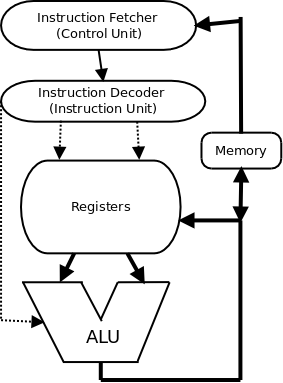
\includegraphics[scale=0.4]{pics/simpleCPU3.png}\\
Figure 1. General microprocessor schema
\end{center}

However our implementation differs from existing ones. It is pretty simple and have one units bilt-in the other units, for example, we don't have separate selfseficient Program Counter. This will be shown in details in next section.\\ 

\newpage
\section{CPU implementation}
\subsection{Instruction Set Architecture}
As it was mentioned in the previous section, ISA defines all specifications of a CPU. In this project we decided to stop on 16bit instructions, that have the same lenght as word, so that we didn't have to think about instructions consisting of more than one word and thus we didn't need to deal with proper splitting of the instruction, which also makes Instruction Unit (our "instruction breaker", decoding in this particular case in easy to perform with obvious rules) easier to implement.
\begin{verbatim}
general specifications:
	16 bit instructions
	16 bit words
	14 registers:
		8 general purpose registers
		6 special purpose registers
\end{verbatim}
The CPU in our implementation uses only one type of instructions, also we don't have special flags. Instead of special flags we use special purpose registers and certain instructions. As already was mentioed: we have implemented pretty simple microprocessor.
\begin{center}
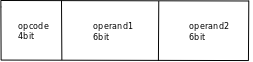
\includegraphics[scale=0.7]{pics/instruction1.png}\\
figure 2. Instruction type
\end{center}
Because we have set the lenght of opcode to 4 bits, we could have only 16 = $2^{4}$ But we have 16 opcodes for "real" instructions and 18 "pseudo" instructions without an opcode, but they are replaced with a composition of the actual instructions (sequence of actual instructions that leads to the same result). For example, an instruction "add" opeartes with two registers, saving result of the operation to the left (or to the first) register:
\begin{verbatim}
movi a 5
movi b 4
add a b
stop
\end{verbatim}
This program will result in:
\begin{verbatim}
program start
PC0 => movi a 7
PC1 => movi b 4
PC2 => add a b
program end
--------------------
registers:
zero: 0
pc: 3
cmp_result: 0
jmp_next: 0
tmp1: 0
tmp2: 0
a: 11
b: 4
c: 0
d: 0
e: 0
f: 0
g: 0
h: 0
\end{verbatim}
In this example  example all registers, that we have are shown, later on only registers that get some value will be shown. "Program end" - is our "stop" instruction (Mostly known as HALT). As the result register "a" gets the value 11 = 7 + 4. We didn't implement any special output register, because we can always store (or move to desirable "output"-register) data manually to certain location in the memory, that we agreed will hold the final result.\\
Both only actual instruction list and all-instruction list can be found in our isa.txt file.\\
Pseudo instructions as we already said can be represented by composition of actual instructions. Some of them consist of two instructions, some of them contain up to 5 instructions. For example:
\begin{verbatim}
movi a 7
addi a 5
stop
\end{verbatim}
The original program consist of 3 instructions, but it results in program with 4 instructions, because addi is a pseudo instruction and it consist of composition of  movi and add instructions.
\begin{verbatim}
program start
PC0 => movi a 7
PC1 => movi tmp1 5
PC2 => add a tmp1
program end
--------------------
\end{verbatim}
Another example for a pseudo instruction would be "modulo" program, 45 mod 10 = 5
\begin{verbatim}
movi a 45
movi b 9
mod a b
stop
\end{verbatim}
But it will result in:
\begin{verbatim}
program start
PC0 => movi a 45
PC1 => movi b 10
PC2 => mov tmp1 a
PC3 => div a b
PC4 => mul a b
PC5 => sub tmp1 a
PC6 => mov a tmp1
program end
--------------------
registers:
pc: 7
tmp1: 5
a: 5
b: 10
\end{verbatim}
Apart from instructions (opcodes) and general information ISA gives information about REGISTERS: general and special purpose.
\begin{verbatim}
registers:
	zero 		000000 # always returns value 0
	
	pc			000001 # program counter
	cmp_result  000010 # result of comparison as defined below
	jmp_next    000011 # je will go here if the comparison succeeds
	tmp1        000100 # temporary register to be used by compiler
	tmp2		000101 # another temporary register

	# general purpose registers
	a       	000110
	b       	000111
	c      	 	001000
	d       	001001
	e       	001010
	f       	001011
	g      	 	001100
	h       	001101
\end{verbatim}
In our project we have decided not to implement both ALU and CU (actually, at the beginning we tried to implement all units separately and then unite them inside of the Control Unit, but we have run into difficulties), but to bild them in into the Control Unit.\\
Execution of a programm in our case goes through following stages:
\begin{enumerate}
	\item[1.] Encode - assembly programm is "translated" with the help of the Assembler module to binary string. The output file gets an extention ".o" and consist of N 16bit strings, where N is a number of "actual instructions" (here, if pseudo instruction is used in the programm, it is translated into several actual instructions for further executing). So, as the result we get "Machine Code".
	\item[2.] Decode - every instruction in output file is split into 3 parts: opcode, operand1 and operand2 accordingly to the number of bits specified in ISA. As the result of this stage we get executable instructions, where the Control Unit knows what operations with what operands to be performed. 
	\item[3.] Execution - is an actual performing of the operations with the given values, using both memory and registers accordingly to the originally written .asm programm. As the result of the executing of a program we get the result "stored" in desirable memory location or register (if specified in the program), or by default in the last "mentioned" left register.\\
Our CPU can be presented as the following schema:
\end{enumerate} 
\begin{center}
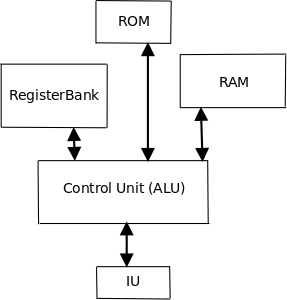
\includegraphics[scale=0.6]{pics/ourCPU.png}\\
Figure 3. Our CPU schema
\end{center}

\newpage
\subsection{Assembler}
As it was mentioned earlier, our first stage of the program execution is the encoding of the program. This happens in assempler.py unit in following order:
\begin{enumerate}
	\item[1.] First, the file with .asm extention is opend into source file for reading, splited into root and extenion. And binary file is created with extention .o.
	\item[2.] This binary file for every code line	"translates" human code into bit-string, that machine can interprete.
	\item[3.] Depending on type of instruction, whether it is an actual or pseudo instruction, the command will be converted into 1 or more bit-strings. (examples of pseudo instructions are given above). Every bit-string is added to the binary file. As the result we get a list containing N bit-strings. You have seen the execution of the program with pseudo instruction (Modulus program). Lower you can see the encoded "machine code". 
\end{enumerate}
For example with modulus binary file will look like this:
\begin{verbatim}
alisa@comrade ~/u/proj> python2 assembler.py programs/test.asm
['0100000110101101', '0100000111001001', '0011000100000110',
 '1000000110000111', '0111000110000111', '0110000100000110',
 '0011000110000100', '0000000000000000']
\end{verbatim} 
Our Assembler contains "translating rules" for all instructions mentioned in the ISA, so that the Control Unit (in our case also ALU) deals only with actual opcodes and executes only them, since in the CU we deal with memory locations and sertain values, what can be only possible with exicting opcodes and thus actual instructions - this is the reason why the program becomes bigger during the encoding stage.\\

\subsection{Memory and Registers}
Every Processor has a memory unit - physical device for working with the program. There are two memory types existing: non-volatile (flash memory,  ROM/PROM/EPROM/EEPROM) and volatile (RAM, DRAM).\\
Non-volatile memory is normally used for storing information for long-term use without its change (overwritting is possible, but it requires much more time and thus not efficient for temporary and "local" computations).\\
In our Implementation ROM gets the instructions and gives "the number of actual instruction" back - holds the address of the instructions. ROM is initialized inside the simulation program as well as the Control Unit.\\
In our implementation ROM has 3 parameters: Rom(dout, addr, CONTENT). The first two are pretty clear. The third parameter of ROM is initialized with the help of special function "load\_program(path)",that is implemented in the Control Unit, that loads the program into list of instructions (bitstring) and returns the list of instructions as unsigned shorts. Afterwards every decoded instruction is assigned an  unique integer, which represents certain location (adrress) in static memory.\\
Currently the most commonly used types of a volatile memory (RAM) are static RAM (SRAM) and dynamic RAM (DRAM). But it is mostly hardware (production difference), since we have a simulation only, we didn't have to work with a specific memory type.\\
In this project RAM is limited with 32 memory-cells. Both RAM and ROM can hold value up to 2 to the power of 2. \\
In order to  work with both static and non-static memory bus is used. In modern processors piplinening is used: several actions (reading and writing back the value) can be performed simultaneously.
In the implementation of this project we have only one channel. Single-channeling is mostly the result of our wrong descision made in the very beginning: we decided to implement a register bank along with memory, but we used the naive realization - a list of registers. We could built distinct registers inside of the Control Unit, so that we had access to separate registers without any time dependency (here the dependency between registers at one clk.posedge is meant).\\ 
Apart from the non- and volatile memory we have implemented a Register Bank, that consists of 14 registers splited into two groups: general purpose and special purpose registers.\\
Since our CPU is quite limited, we don't need many registers to work with. We have implemented several special-purpose registers to partially substitute flags and some hardware units. For example we have a "pc-register, that gets/holds the adress of the next instruction directly from the CU (we don't have a selfseficient Program Counter, in our case the number of the next instruction is the number of the line, where particular instruction is located).\\

\subsection{Instruction Unit}
Since we have restricted the lenght of words and instruction size to the same value (16bit, or 2byte), decoding an instruction became really easy:
according to in ISA specified instruction type an opcode gets first 4bit, than an operand1 gets next 6 bit and the last 6bit gets an operand2 (it is also shown in the figure 2). Some opcodes require only one operand ("not"). It is implemented the way, that typing in the second operand (supposed mistyping), does not influence the result and does not throw an error or an emergency program stop, because in the implementation the second operand is ignored.\\
For example:
\newpage
\begin{verbatim}
movi a 3
movi b 9
not a b
stop
\end{verbatim}
Will result in:
\begin{verbatim}
program start
PC0 => movi a 45
PC1 => movi b 9
PC2 => not a
program end
--------------------
registers:
zero: 0
pc: 3
cmp_result: 0
jmp_next: 0
tmp1: 0
tmp2: 0
a: 65533
b: 9
\end{verbatim}
As you can see, the second operand really doesn't influence neither the executing of the program, nor the correctness of the result.\\

\newpage
\subsection{Control Unit}
Classically, the Control Unit (CU) handles the operation of the whole prozessor, it manages communication between in- and output devices, interprets and executes them itself (in our case), or via ALU. Also, the Control Unit provides control signals, like clock (clk in our code). The CU performs all four stages of a program execution.\\
In our project the Control Unit is implemented inside of the cpu-simulation module, and the instances of RAM, ROM; Register Bank and Instruction Unit are controlled by the CU but as separate units (instances are innitialized before the implementation of the Control Unot itself). This leads to some inefficiency, like (already mentioned above) single-threading: one register at a time can be used. The Program Counter, normally is a selfseficient unit that is implemented outside the CU, but in our case is also build-in in the Control Unit. Since we have a special register for the address of the next instruction ("pc"-register), the CU presents two cases changing the value in pc-register. These two cases are:
\begin{enumerate}
	\item[1.] The instruction is already executed, and certain operations are successfully performed. Afterwards the value in the pc-register is just incremeted (in "Memory and Registers" section it was shown how pc tracks the executable insruction and how does ROM is initialized). 
	\item[2.] The second possibility to change the PC is using flow-control instruction (Jump-instructions, see Appendix). These are jump-opcodes. Here in special-purpose register "jmp\_next" the location of the jump (the adress of the next desirable instruction) is stored. If the condition of the jump-operation match the result, the pc gets the value from jmp\_next-register. This way cycles are normally implemented in assembly.	
\end{enumerate} 
The way our CPU works is following:
\begin{enumerate}
	\item[1.] The program, written in Assembly is encoded by assembler.py (concerete examples and explanations are in "assembler" subsection).
	\item[2.] In the module "simulation.py" firts the programm is decoded with function "load\_program(path)"; the result is used as the third parameter for ROM initialization (all instructions in the program get their unique id for futher pc addressing). Also RAM, RegisterBank, Clock and Instruction Unit are initialized for futher operation of the Control Unit.
	\item[3.] In the CU for every instruction an opcode is defined and the proper action is performed with the operands given in the instruction until the opcode "stop" (0000) is reached. All nessussary output is printed.  
\end{enumerate}

\newpage
\section{Results}
\subsection{Test of the CPU}
Now, let us test all features of the CPU and its workability all together with the help of more complicated programm: Euclidean algorithm.\\
Euclidean algorithm is well known algorithm for computing the greatest common divisor (GCD) of two (usually positive) integers, also known as the greatest common factor (GCF) or highest common factor (HCF).\\
The way this algorithm works is:
\begin{verbatim}
function gcd(a, b)
    while b ≠ 0
       t := b
       b := a mod b
       a := t
    return a
\end{verbatim}
The smallest number is substructed from the biggest number until they are equal and a-register holds the GCD.\\
First we need to write the program in assembly:
\begin{verbatim}
0.  movi a 45
1.  movi e 3
2.  movi f 2
3.  movi b 3
4.  shift_l a e
5.  shift_l b f
6.  mov g a
7.  mov h b
8.  movi c 0
9. .loop
10. movi jmp_next .loop
11. mov d b
12. mod a b
13. mov b a
14. mov a d
15. jne b c
16. stop
\end{verbatim}
The Assembly encoding of the program looks like:
\begin{verbatim}
alisa@comrade ~/u/proj> python2 assembler.py programs/ggt.asm
['0100000110101101', '0100001010000011', '0100001011000010',
 '0100000111000011', '1100000110001010', '1100000111001011',
 '0011001100000110', '0011001101000111', '0100001000000000',
 '0100000011001001', '0011001001000111', '0011000100000110',
 '1000000110000111', '0111000110000111', '0110000100000110',
 '0011000110000100', '0011000111000110', '0011000110001001',
 '1110000111001000', '0100000100000001', '1111000100000010',
 '0100000100000010', '1111000100000010', '0000000000000000']
\end{verbatim}
The binary file has 24 instructions because of the several pseudo instructions in the original program. Since the Control Unit in our project deals only with the opcodes of the actual operations assembler writes back the composition of actual instructions for each pseudo instruction used in the code.\\
The next step is simulation of the program, using the output file "ggt.o"
\begin{verbatim}
alisa@comrade ~/u/proj> python2 simulation.py programs/ggt.o
program start
PC0 => movi a 45
PC1 => movi e 3
PC2 => movi f 2
PC3 => movi b 3
PC4 => shift_l a e
PC5 => shift_l b f
PC6 => mov g a
PC7 => mov h b
PC8 => movi c 0
PC9 => movi jmp_next 9
PC10 => mov d b
PC11 => mov tmp1 a
PC12 => div a b
PC13 => mul a b
PC14 => sub tmp1 a
PC15 => mov a tmp1
PC16 => mov b a
PC17 => mov a d
PC18 => cmp b c
PC19 => movi tmp1 1
PC20 => je tmp1 cmp_result
PC21 => movi tmp1 2
PC22 => je tmp1 cmp_result
program end
--------------------
registers:
zero: 0
pc: 23
cmp_result: 0
jmp_next: 9
tmp1: 2
tmp2: 0
a: 12
b: 0
c: 0
d: 12
e: 3
f: 2
g: 360
h: 12
memory:
0: 0    1: 0    2: 0    3: 0
4: 0    5: 0    6: 0    7: 0
8: 0    9: 0    10: 0   11: 0
12: 0   13: 0   14: 0   15: 0
16: 0   17: 0   18: 0   19: 0
20: 0   21: 0   22: 0   23: 0
24: 0   25: 0   26: 0   27: 0
28: 0   29: 0   30: 0   31: 0
\end{verbatim}
The result of the program is stored in the first used operand in opcode "mod" (pretty much the core function of the algorithm). The register "a" has value = 12, that is indeed the GCD of 360 (shift\_l 45 3) and 12 (shift\_l 3 2).\\
In this program we havn't used RAM (but we could potentialy run the computation through the memory or keep some result there).
Also, in order to see the clock synchronization, you can look on the wave diagram of the project:\\
\begin{center}
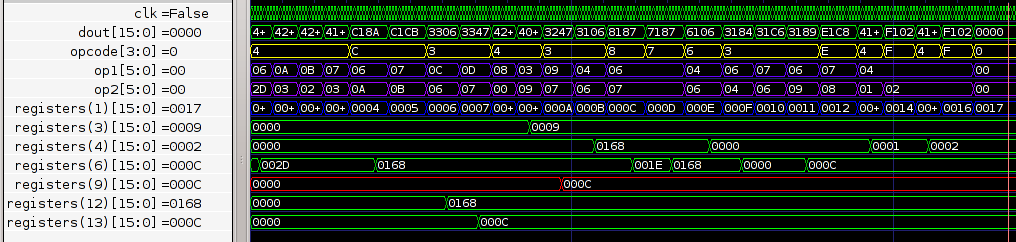
\includegraphics[scale=0.5]{pics/gtkwave.png}\\
Figure 4. GTK Wave
\end{center}			
			
\newpage
\subsection{Possible improvements}
During the realisation of the project we have used MyHDL, which is python2 library for VHDL (also converting to verilog is possible). According to choosen language we had some restrictions and run into some difficulties.\\
The first difficulty was the synchronizing. In the beginning we decided to implement "classical" circuit - all units had to be implemented seperatly (distinct unit on a circuit), but we ran into asynchronious work of all units when uniting them in simulation module. According to naive implementation we had multiple cloks. This problem was decided by substituting multiple units with memory units (includong registers), encoding unit (IU) and built-in CU in the simulation modul with main clock initializing\\
Next difficulty was single-threading. It is not a problem for a university project, but pottentially such slow COU won't be produced (In fact modern micro processors are multi-threaded). This is mostly the consequence of the not optimal architecture, that we have chosen. By implementing each register-cell seperatly in the simulation mode will give us opportunity to use all of them in one tick and would reduce amount of code and needed tricks inside of Control Unit implementation.\\
The obvious limitation for word- and instruction-size gave us pseudo instructions-problem. This results in extending of the program for several additional instructions and thus increasing the time the program needs to be completely executed. But at the same time it was some sort of hack for increasing amount of commands from 16 to 34, that increased the amount of possible program executing of our CPU.\\
But overall our simple CPU can perform simple and middle-difficult math operations, algorithms. 

\newpage
\section*{Appendix}
\subsection*{ISA}
\begin{tabular}{|c|c|c|c|}
\hline
\multirow{11}{*}{Arithmetic} & add & add a b & 0101 000110 000111 \\
& addi & addi a 3 & pseudo \\
& sub & sub a b & 0110 000110 0000111\\
& subi & subi a 6 & pseudo\\
& mul & mul a b & 0111 000110 0000111\\
& muli & muli a 2 & pseudo\\
& div & div a b & 1000 000110 0000111\\
& divi & divi a 3 & pseudo\\
& inc & inc a b & pseudo\\
& dec & dec a 3 & pseudo\\
& swap & swap a b & pseudo\\
\hline
\multirow{6}{*}{Logical} & not & not a & 1001 000110 000000\\
& and & and a b & 1010 000110 000111\\
& or & or a b & 1011 000110 000000\\
& xor & xor a b & pseudo\\
& nand & nand a b & pseudo\\
& nor & nor a b & pseudo\\
\hline
\multirow{2}{*}{Shift} & shifl\_l & shift\_l a b & 1100 000110 000111\\
& shifl\_r & shift\_r a b & 1101 000110\\
\hline
\multirow{7}{*}{Jump} & j & j & pseudo \\
& je & je a b & 1111 000110 000111 \\
& jne & jne a b & pseudo \\
& jg & jg a b & pseudo \\
& jge & jge a b & pseudo \\
& jl & jl a b & pseudo \\
& jle & jle a b & pseudo \\
\hline
\multirow{4}{*}{Memory} & store & store a b & 0001 000110 000111\\
& load & load a b & 0010 000110 000111\\
& mov & mov a b & 0011 000110 000111\\
& movi & movi a 5 & 0001 000110 000101\\
\hline
\multirow{2}{*}{Flow} & stop & stop & 0000 000000 000000 \\
& noop & noop & pseudo \\
\hline
\end{tabular}
\end{document}

